\section{Introduction}
\label{sec:introduction}

\section*{Intro guidance}

Just to clarify the goal of this project is to use kinematic maps to ascertain if the post-starburst galaxies are caused by mergers (i.e. post-mergers). 

There are another couple of papers to look at:
Stark et al. 2018: \citep{2018MNRAS.480.2217S} 
Barrera-Ballesteros et al. 2015: \citep{2015A&A...582A..21B}
 
Once you have looked at these, could you move up and down the references and cited papers in each paper, and see if you can find any other methods that have been used to identify merger or post-merger features \textbf{using kinematic features or maps}?
 
Extend your report to perhaps 1.5-2 pages to give a complete summary of the literature.

On discussion with Anne-Marie, we are not convinced that the full kinemetry fits will provide useful data on MaNGA galaxies. Note that it is important to get good marks on your final report that you provide a critical assessment of both your results and previous results, so have a think about the methods and what might work / not work on the MaNGA galaxies. 

\vspace{6pt}
\textbf{Remember to remove redundant subsection outlining placeholders.}


\subsection{SDSS IV MaNGA}
An overview of the SDSS MaNGA project is provided by \citet{2015ApJ...798....7B}. A concise description of the \href{https://iopscience.iop.org/article/10.1088/0004-637X/798/1/7/meta#apj504473s3}{survey design} is included in Section 3. \citet{2008MNRAS.388.1321P} have analysed the distribution of galaxy shapes in the SDSS DR6. The shapes of high-redshift galaxies has been investigated by \citet{2012ApJ...754L..24C}.

\subsection{Post-starburst (PSB) Galaxies}
\label{sec:PSBs}
Vivienne has been involved in the preparation of a number of papers researching PSBs: \citet{2017MNRAS.472.1401A} regarding the relationship between quenching of star formation and morphological transition, while \citet{2016MNRAS.463..832W} sets out the background work.
\par Galaxy evolution has been explained by many authors [TODO: expand to create a list] \citep{baldry2004quantifying,2006MNRAS.373..469B} by referring to a galaxy colour-magnitude diagram (CMD) as illustrated in Fig.~\ref{fig:CMD1}. Young, late-type blue, often spiral galaxies in the lower-right 'blue cloud' region are understood to transition to the redder mainly early-type elliptical galaxies along the upper left 'red sequence' region of the CMD. There is a sparsely populated region separating the two populations: this is often referred to as the 'green valley' region. In this paper we explore galaxies in transition between the blue cloud and the red sequence, through the green valley.

\begin{figure}
	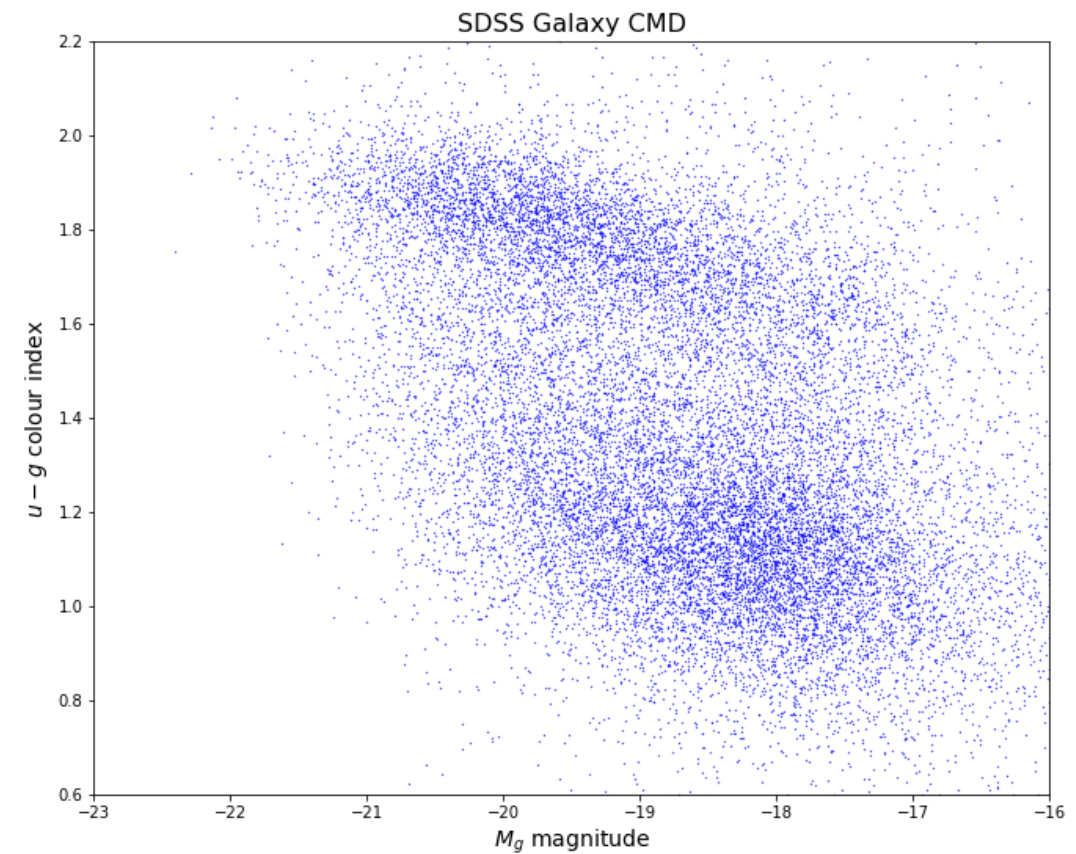
\includegraphics[width=\columnwidth]{images/CMDs/galaxyCMD.PNG}
    \caption{Galaxy colour-magnitude diagram: $u-g$ colour index versus $M_g$ magnitude. The bimodality of the distribution is discussed in the text.}
    \label{fig:CMD1}
\end{figure}

\subsection{Structure}
The content of the paper is organised as follows: Section \ref{sec:sample} describes the conditions required for PSB sample and the corresponding control galaxies. Data analysis methods are discussed in Section \ref{sec:analysis}. Finally, a summary of the research and the conclusions drawn from this work, along with recommendations for further study are presented in Section \ref{sec:discussion}.
